% Copyright 2008 by Mark Wibrow
%
% This file may be distributed and/or modified
%
% 1. under the LaTeX Project Public License and/or
% 2. under the GNU Free Documentation License.
%
% See the file doc/generic/pgf/licenses/LICENSE for more details.

\section{Decoration Library}
\label{section-library-decorations}

\begin{pgflibrary}{decorations}
  This library package defines basic decorations.
  Section~\ref{section-tikz-snakes-and-decorations} explains how
  decorations are used in \tikzname,
  Section~\ref{section-base-snakes-and-decorations}   explains how new
  snakes can be defined. 

  The decorations are influenced by the current values of keys like
  |/pgf/decoration segment amplitude|. Meta-decorations are influenced
  by the values of keys like |/pgf/meta-decoration segment amplitude|.
\end{pgflibrary}

\begin{decoration}{zigzag}
	This decoration looks like a zig-zag line. The following parameters
  influence the decoration:
  \begin{itemize}
  \item |/pgf/decoration segment amplitude|
    determines how much the zig-zag lines raises above and falls below
    a straight line to the target point.
  \item |/pgf/decoration segment length|
    determines the length of a complete ``up-down'' cycle.
  \end{itemize}
\begin{codeexample}[]
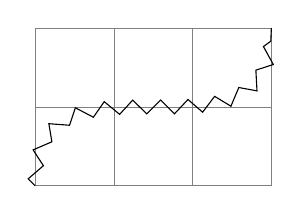
\begin{tikzpicture}[decoration=zigzag]
  \draw [help lines] grid (3,2);
  \draw [decorate] (0,0) .. controls (0,2) and (3,0) .. (3,2);
\end{tikzpicture}
\end{codeexample}
\end{decoration}

\begin{decoration}{saw}
	This decoration looks like the blade of a saw. The following parameters
  influence the decoration:
  \begin{itemize}
  \item |/pgf/decoration segment amplitude|
    determines how much each spike raises above the straight line.
  \item |/pgf/decoration segment length|
    determines the length each spike.
  \end{itemize}
\begin{codeexample}[]
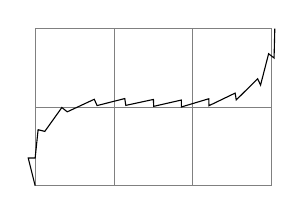
\begin{tikzpicture}[decoration=saw]
  \draw [help lines] grid (3,2);
  \draw [decorate] (0,0) .. controls (0,2) and (3,0) .. (3,2);
\end{tikzpicture}
\end{codeexample}
\end{decoration}

\begin{decoration}{triangles}
	This decoration adds triangles to the path that point toward the
  target. The following parameters influence the decoration: 
  \begin{itemize}
  \item |/pgf/decoration segment length|
    determines the distance between consecutive triangles.
  \item |/pgf/decoration segment amplitude|
    determines half the length of the triangle side that is orthogonal
    to the path.
  \item |/pgf/decoration segment object length|
    determines the height of the triangle.
  \end{itemize}
\begin{codeexample}[]
\begin{tikzpicture}[decoration=triangles]
  \draw [help lines] grid (3,2);
  \draw [decorate] (0,0) .. controls (0,2) and (3,0) .. (3,2);
\end{tikzpicture}
\end{codeexample}
\end{decoration}

\begin{decoration}{crosses}
	This decoration adds (diagonal) crosses to the path. The following
  parameters influence the decoration:  
  \begin{itemize}
  \item |/pgf/decoration segment length|
    determines the distance between consecutive crosses.
  \item |/pgf/decoration segment amplitude|
    determines half the hieght of each cross.
  \item |/pgf/decoration segment object length|
    determines width of each cross.
  \end{itemize}
\begin{codeexample}[]
\begin{tikzpicture}[decoration=crosses]
  \draw [help lines] grid (3,2);
  \draw [decorate] (0,0) .. controls (0,2) and (3,0) .. (3,2);
\end{tikzpicture}
\end{codeexample}
\end{decoration}

\begin{decoration}{ticks}
  This decoration adds straight lines  the path that are orthogonal to 
  the line toward the target. The following parameters influence the 
  decoration: 
  \begin{itemize}
  \item |/pgf/decoration segment length|
    determines the distance between consecutive ticks.
  \item |/pgf/decoration segment amplitude|
    determines half the length of the ticks.
  \end{itemize}
\begin{codeexample}[]
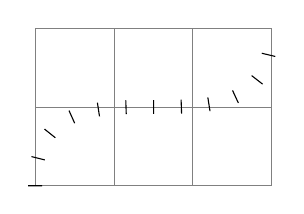
\begin{tikzpicture}[decoration=ticks]
  \draw [help lines] grid (3,2);
  \draw [decorate] (0,0) .. controls (0,2) and (3,0) .. (3,2);
\end{tikzpicture}
\end{codeexample}
\end{decoration}

\begin{decoration}{text}
  This decoration decorates the path with text.
	
\begin{codeexample}[]
\catcode`\|12
\begin{tikzpicture}
  \draw [help lines] grid (3,2);
  \draw [red, dashed, postaction={decoration=text, decorate,
    decoration text={Some text along a curve}}] 
    (0,0) .. controls (0,2) and (3,0) .. (3,2);
\end{tikzpicture}
\end{codeexample}

  \pgfname{} ``does its best'' to typeset the text, however you
  should note the following points:
  \begin{itemize}
  \item
    Each character in the text is typeset in a separate |\hbox|. This
    means that if you want fancy things like kerning or ligatures you
    will have to manually annotate the characters in the decoration 
    text within a group, for example, |W{\kern-1ptA}TER|. 
  \item
    Each character is positioned using the center of its baseline. To
    move the text vertcally (relative to the path), the additional
    transform key should be used.
  \item
    No attempt is made to ensure characters do not overlap when
    the angle between segments is considerably less than 180\textdegree{}
    (this is tricky to do in \TeX{} without a huge processing
    overhead). In general this should not be too much of a problem, 
    but, once again, kerning can be used in most cases to overcome 
    any undesirable	effects.
  \item			
    It is only possible to typeset text in math mode under considerable
    restrictions. Math mode is entered and exited using any character	
    of category code 3 (e.g., in plain \TeX{} this is |$|). %$
    Math subscripts and superscripts need to be	contained within braces 
    (e.g., |{^y_i}|) as do commands like |\times| or |\cdot|. 
    However, even modestly complex mathematical	typesetting is unlikely 
    to be sucessful along a path (or even desirable).
  \item
    Some inaccuracies in positioning may be particularly apparent
    at subpath boundaries. This can (unfortunately) only be solved 
    on case by case basis	by individually kerning the offending 
    characters within a group.
  \end{itemize}
  
  The following keys are used by the |text| decoration:
  
  \begin{key}{/pgf/decoration text=\marg{text} (initially \char`\{\char`\})}
    Set the text to typeset along the curve. 
    Consecutive spaces are ignored, so |\ | (or |\space| in \LaTeX) 
    should be used to insert multiple spaces.	It is possible to
    format the text using normal formating commands, such as |\it|, |\bf|
    and |\color|, within customisable delimiters. Initially these
    delimiters are both {\tt\char`\|} (however, care will be needed 
    regarding	the category codes of delimiters --- see below). 

{\catcode`\|12
\begin{codeexample}[]
\catcode`\|12
\begin{tikzpicture}
  \draw [help lines] grid (3,2);
  \path [decorate, decoration=text,	
   decoration text={a big |\color{green}|green|| juicy apple.}] 
    (0,0) .. controls (0,2) and (3,0) .. (3,2);
\end{tikzpicture}
\end{codeexample}
}
  By following the first delimiter
  with |+|, the formatting commands are added to any exisiting 
  formatting.

{\catcode`\|12
\begin{codeexample}[]
\begin{tikzpicture}
  \draw [help lines] grid (3,2);
  \path [decorate, decoration=text,	
     decoration text={a |\large|big |+\bf\color{red}|red|| juicy apple.}] 
    (0,0) .. controls (0,2) and (3,0) .. (3,2);
\end{tikzpicture}
\end{codeexample}
}
	
  Internally, the text is stored in the macro |\pgfdecorationtext|. 
  Any characters that have not been typeset when the end of the 
  path has been reached will be stored in |\pgfdecorationrestoftext|.

\end{key}

{\catcode`\|12
\begin{key}{/pgf/decoration text format delimiters=\marg{before}\marg{after} (initially \char`\{|\char`\}\char`\{\char`\})}

  \catcode`\|13
	
  Set the characters that the text decoration will use to parse 
  formatting commands. 
  If \meta{after} is empty, then \meta{before} will be used for both
  delimiters.
  In general you should stick to characters	whose category codes are 
  |11| or |12|.
  As |+| is used to indicate that the specifed format commands 
  are added	to any exisiting ones, you should avoid using |+| as
  a delimiter. 

\begin{codeexample}[]
\begin{tikzpicture}
  \draw [help lines] grid (3,2);
  \path [decorate, decoration=text, decoration text format delimiters={[}{]}, 
  decoration text={A big [\color{red}]red[] and [\color{green}]green[] apple.}] 
    (0,0) .. controls (0,2) and (3,0) .. (3,2);
\end{tikzpicture}
\end{codeexample}
\end{key}
}

\begin{key}{/pgf/decoration text color=\meta{color} (initially black)}
  Set the color for the text.
\end{key}
\end{decoration}

\begin{meta-decoration}{lineto zigzag}
  This meta-decoration decorates the path by alternating between 
  |lineto| and |zigzag| decorations. It always finishes
  with the |lineto| decoration. The parameters for the |zigzag|
  decoration are set in the usual manner (see above).	
  This meta-decoration depends on
  the following parameter:
	
  \begin{itemize}
  \item	|/pgf/meta-decoration segment length|
    determines how far each decoration decorates the path.
  \end{itemize}

\begin{codeexample}[]
\begin{tikzpicture}
  \draw [help lines] grid (3,2);
  \draw [meta-decoration=lineto zigzag, meta-decoration segment length=0.5cm,
         decoration options={segment length=.125cm}] 
    decorate {(0,0) .. controls (0,2) and (3,0) .. (3,2)};
\end{tikzpicture}
\end{codeexample}
\end{meta-decoration}

